\input{../template/style.tex}

\hypersetup{hidelinks}

% Cross-region DAG execution for latency-sensitive pipelines
\graphicspath{{papers/Orchestrating_Near_Exchange_Compute/}}

% Extra packages.
\usepackage{microtype}
\usepackage{doi}
\usepackage{url}
\usepackage{booktabs}
\usepackage{tabularx}
\usepackage{amsmath}
\usepackage{listings}
\usepackage{xcolor}
\usepackage{tikz}
\usepackage{float}
\usepackage[font=small, labelfont=bf]{caption}
\usetikzlibrary{arrows.meta, positioning, calc, fit, backgrounds}

\setlength{\emergencystretch}{2em}

% Calm listings style.
\definecolor{CausifyBg}{RGB}{248,248,248}
\definecolor{CausifyFrame}{RGB}{220,220,220}
\definecolor{CausifyComment}{RGB}{110,110,110}
\definecolor{CausifyKeyword}{RGB}{36,74,140}
\definecolor{CausifyString}{RGB}{24,110,90}
\definecolor{CausifyNumber}{RGB}{125,125,125}

\lstdefinestyle{causify}{
  basicstyle=\ttfamily\footnotesize,
  backgroundcolor=\color{CausifyBg},
  frame=single,
  rulecolor=\color{CausifyFrame},
  framerule=0.4pt,
  framesep=6pt,
  xleftmargin=\parindent,
  xrightmargin=\parindent,
  numbers=left,
  numberstyle=\tiny\color{CausifyNumber},
  numbersep=8pt,
  keywordstyle=\bfseries\color{CausifyKeyword},
  commentstyle=\itshape\color{CausifyComment},
  stringstyle=\color{CausifyString},
  showstringspaces=false,
  breaklines=true,
  breakatwhitespace=true,
  postbreak=\mbox{\textcolor{CausifyNumber}{$\hookrightarrow$}\space},
  tabsize=2,
  columns=fullflexible,
  keepspaces=true,
  captionpos=b,
  aboveskip=0.8\baselineskip,
  belowskip=0.8\baselineskip
}

\lstdefinestyle{python}{
  style=causify,
  morekeywords={def,class,if,else,elif,for,while,return,import,from,as,try,except,finally,with,lambda,yield,assert,pass,break,continue,in,is,not,and,or,True,False,None,async,await}
}
\lstdefinestyle{json}{style=causify,morestring=[b]"}

% Macros
\newcommand{\system}{\textsc{Causify Trading Platform}}
\newcommand{\airflow}{\textsc{Airflow}}
\newcommand{\ecs}{\textsc{ECS}}
\newcommand{\fargate}{\textsc{Fargate}}
\newcommand{\nearEx}{\emph{near-exchange}}
\newcommand{\regionAware}{\emph{region-aware}}
\renewcommand{\dag}{\textsc{DAG}}

\begin{document}
  \title{Orchestrating Near-Exchange Compute:\\ \large Cross-Region \dag{}
  Execution for Latency-Sensitive Pipelines}

  % \author{\textbf{[Author Name]}\\ % [Affiliation]\\ % \texttt{[email]}}

  \date{\today}

  \begin{abstract}
    Latency-sensitive pipelines are allergic to geography. When data is
    produced in one place (an exchange endpoint) and consumed in another
    (a trading system), the round-trip time between regions becomes part
    of the model---and sometimes part of the P\&L. Traditional high-frequency
    trading solves this with co-location and bespoke networks. In cloud-native
    systems, we approximate the same intent by running compute \nearEx{}:
    close to the source, close to the consumers, and close to the
    storage that must be updated.

    We describe a production pattern for \regionAware{} workflow orchestration:
    a single \airflow{} scheduler coordinates containerized tasks executed
    in multiple AWS regions. Workloads are launched via \ecs{} \fargate{}
    using \airflow{}'s \texttt{EcsRunTaskOperator}, extended with a retry
    strategy that handles common capacity and provisioning failures.
    Region selection is encoded in the \dag{} naming convention and automatically
    mapped to execution region, VPC networking, and region-specific shared
    storage mounts. The same orchestration fabric powers high-rate
    websocket ingestion, archival to object storage, resampling, QA, and
    scheduled trading observers---all while keeping the scheduler stable
    and the execution substrate elastic.

    We present the architecture, the contract points between scheduler and
    workers, the reliability fixes that turned theory into operations, and
    an evaluation methodology for measuring end-to-end knowledge latency.
    We also discuss limitations and future directions, including hardware-assisted
    near-zero-latency paths.
  \end{abstract}

  \maketitle

  \setcounter{tocdepth}{1}
  \tableofcontents

% ##############################################################################
  \section{Introduction}
  In latency-sensitive systems, ``fast'' is not a benchmark result; it is
  a product feature. A model is only as fresh as its inputs, and in trading,
  freshness competes directly with other people's freshness. The hard part
  is rarely compute. The hard part is the path: network hops, queueing, scheduling,
  and the silent tax of cross-region requests.

  The classic response in high-frequency trading is co-location: bring compute
  to the exchange. Cloud platforms do not give you a rack next to a
  matching engine, but they do give you regions. That is enough to
  reframe the problem as \emph{placement}: run collectors and short-lived
  jobs in the region that minimizes latency to the source, and keep the orchestration
  control plane simple enough that it never becomes the bottleneck.

  This paper describes how \system{} implemented \regionAware{} orchestration:
  \begin{itemize}
    \item \airflow{} runs as a stable scheduler (control plane) and
      remains region-agnostic.

    \item Tasks execute as containers on \ecs{} \fargate{} in multiple regions
      \cite{airflow_ecs_operator,aws_ecs_runtask,aws_fargate_networking}.

    \item Region selection is derived from \dag{} names (e.g.,
      \texttt{preprod.tokyo.*} vs \texttt{preprod.europe.*}) and mapped to
      AWS region, VPC networking, and region-specific mounts.

    \item Reliability is engineered explicitly: retries for \ecs{} start
      failures and provisioning delays, large waiter bounds, and operational
      rollouts by region.
  \end{itemize}

  \paragraph{Contributions.}
  \begin{itemize}
    \item A practical pattern for \regionAware{} orchestration with a
      single scheduler and multi-region execution.

    \item A \emph{filename-as-configuration} approach that encodes
      region and dataset identity into \dag{} names, enabling simple
      automation.

    \item An operationally motivated extension of \texttt{EcsRunTaskOperator}
      that handles common \ecs{} failure modes \cite{airflow_ecs_operator,airflow_amazon_exceptions}.

    \item A measurement framework for end-to-end \emph{knowledge latency}
      (when a data point becomes usable), not just network RTT.
  \end{itemize}

% ##############################################################################
  \section{Background and Problem Statement}

% ==============================================================================
  \subsection{Why geography dominates}
  Let $T$ be the end-to-end time from an exchange update to a queryable record
  in the database. A useful decomposition is:
  \[
    T \approx T_{\text{network}}+ T_{\text{collector}}+ T_{\text{queue}}+
    T_{\text{db}}+ T_{\text{availability}}.
  \]
  Cross-region workflows inflate $T_{\text{network}}$ and often $T_{\text{queue}}$
  (due to additional hops and contention). The physics is unforgiving: propagation
  delay is bounded by the speed of light and the path length \cite{singla_speed_of_light,bhattacherjee_fast_networks}.
  The engineering is similarly unforgiving: even when messages are small,
  micro-bursts and retries accumulate into visible lag.

% ==============================================================================
  \subsection{Why \airflow{} + \fargate{}}
  We choose \airflow{} for orchestration because it gives: (i) a mature
  scheduling model, (ii) explicit dependencies, and (iii) operational
  visibility. We choose \fargate{} because we want burst compute without
  cluster debt: tasks can scale up, run, and disappear. Most importantly,
  \fargate{} tasks can be launched in the region closest to the data
  source, while the scheduler stays put.

% ==============================================================================
  \subsection{Design goals}
  We build toward five goals:
  \begin{enumerate}
    \item \textbf{G1 (Near-exchange placement):} execute collectors and
      latency-critical jobs in regions closest to the exchange endpoints.

    \item \textbf{G2 (Single scheduler):} keep one \airflow{} scheduler to
      avoid multi-scheduler drift and duplicated operational overhead.

    \item \textbf{G3 (Deterministic region selection):} derive region
      from \dag{} identity, not ad-hoc operator parameters.

    \item \textbf{G4 (Reliability under real failures):} handle the \ecs{}
      failures that happen in production (capacity, ENI provisioning,
      ephemeral storage) with explicit retries.

    \item \textbf{G5 (Measurable latency):} define and measure \emph{knowledge
      latency}, not just transport latency.
  \end{enumerate}

% ##############################################################################
  \section{Architecture Overview}

% ==============================================================================
  \subsection{Two planes: orchestration vs execution}
  This system is a control-plane/data-plane split applied to workflows:
  \begin{itemize}
    \item \textbf{Orchestration plane:} Airflow parses DAGs, schedules tasks,
      enforces dependencies, emits logs/metrics.

    \item \textbf{Execution plane:} tasks run as containers on ECS/Fargate
      in one of several AWS regions.
  \end{itemize}
  The critical bridge between the planes is \emph{region selection}. We
  encode it in a way that scales with the number of DAGs: a naming convention
  and a parser.

% ==============================================================================
  \subsection{Region selection: filename-as-configuration}
  DAG filenames follow a structured convention that includes the location
  token: \texttt{tokyo} or \texttt{europe}. At parse time, the system
  maps this token to:
  \begin{itemize}
    \item AWS region (e.g., \texttt{ap-northeast-1} vs \texttt{eu-north-1}),

    \item region-specific VPC networking (subnets, security groups,
      public IP assignment),

    \item region-specific mounts/paths used by tasks.
  \end{itemize}

  This approach deliberately keeps region selection \emph{out} of ad-hoc
  operator kwargs and \emph{out} of task code. The DAG identity is the source
  of truth.

% ==============================================================================
  \subsection{Cross-region execution flow}
  Figure~\ref{fig:arch} shows the end-to-end flow. The scheduler stays
  centralized; tasks fan out to regions.

  \begin{figure}[H]
    \centering
    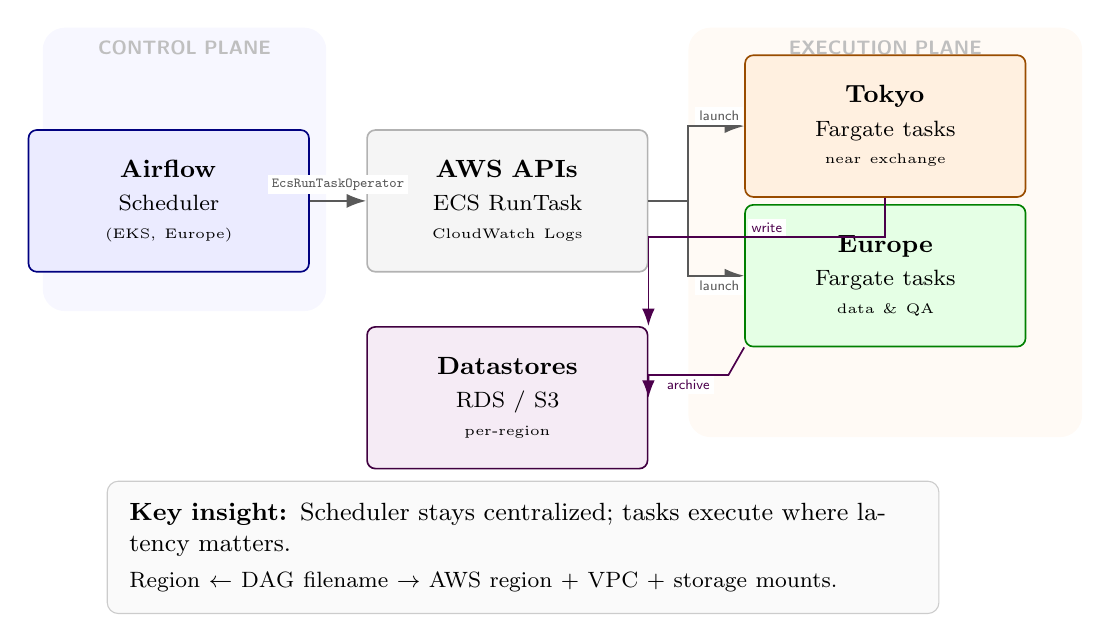
\begin{tikzpicture}[
      controlcol/.style={fill=blue!8, draw=blue!50!black, line width=0.6pt},
      exectokyocol/.style={fill=orange!12, draw=orange!60!black, line width=0.6pt},
      execeurocol/.style={fill=green!10, draw=green!50!black, line width=0.6pt},
      apicol/.style={fill=gray!8, draw=gray!60, line width=0.6pt},
      storecol/.style={fill=violet!8, draw=violet!50!black, line width=0.6pt},
      mainbox/.style={draw, rounded corners=3pt, align=center, inner sep=8pt, text width=30mm, minimum height=18mm, font=\small},
      arrow/.style={-{Latex[length=2.5mm, width=1.8mm]}, line width=0.7pt, gray!70!black},
      dataarrow/.style={-{Latex[length=2.2mm, width=1.6mm]}, line width=0.6pt, violet!60!black},
      lab/.style={font=\scriptsize\sffamily, align=center, fill=white, inner sep=1.5pt},
      planelabel/.style={font=\scriptsize\sffamily\bfseries, text=gray!50}
    ]
      % Control Plane background
      \begin{scope}[on background layer]
        \fill[blue!3, rounded corners=8pt]
          (-1.6,-1.4) rectangle (2.0,2.2);
      \end{scope}
      \node[planelabel] at (0.2,1.95) {CONTROL PLANE};

      % Execution Plane background
      \begin{scope}[on background layer]
        \fill[orange!4, rounded corners=8pt]
          (6.6,-3.0) rectangle (11.6,2.2);
      \end{scope}
      \node[planelabel] at (9.1,1.95) {EXECUTION PLANE};

      % Main nodes
      \node[mainbox, controlcol]
        (airflow)
        at
        (0,0)
        { \textbf{\airflow{}}\\[1pt] {\footnotesize Scheduler}\\[-1pt] {\tiny (EKS, Europe)} };

      \node[mainbox, apicol]
        (api)
        at
        (4.3,0)
        { \textbf{AWS APIs}\\[1pt] {\footnotesize ECS RunTask}\\[-1pt] {\tiny CloudWatch Logs} };

      \node[mainbox, exectokyocol]
        (tokyo)
        at
        (9.1,0.95)
        { \textbf{Tokyo}\\[1pt] {\footnotesize Fargate tasks}\\[-1pt] {\tiny near exchange} };

      \node[mainbox, execeurocol]
        (europe)
        at
        (9.1,-0.95)
        { \textbf{Europe}\\[1pt] {\footnotesize Fargate tasks}\\[-1pt] {\tiny data \& QA} };

      \node[mainbox, storecol]
        (db)
        at
        (4.3,-2.5)
        { \textbf{Datastores}\\[1pt] {\footnotesize RDS / S3}\\[-1pt] {\tiny per-region} };

      % Control flow arrows
      \draw[arrow]
        (airflow.east) --
        node[lab, above=2pt] {\tiny\texttt{EcsRunTaskOperator}}
        (api.west);
      \draw[arrow]
        (api.east) --
        ++(0.5,0) |-
        node[lab, above, pos=0.78] {\tiny launch}
        (tokyo.west);
      \draw[arrow]
        (api.east) --
        ++(0.5,0) |-
        node[lab, below, pos=0.78] {\tiny launch}
        (europe.west);

      % Data flow arrows (to datastores)
      \draw[dataarrow]
        (tokyo.south) --
        ++(0,-0.5) -|
        node[lab, above, pos=0.25] {\tiny write}
        (db.north east);
      \draw[dataarrow]
        (europe.south west) --
        ++(-0.2,-0.35) -|
        node[lab, below, pos=0.25] {\tiny archive}
        (db.east);

      % Key insight box at bottom
      \node[
        draw=gray!40,
        fill=gray!4,
        rounded corners=4pt,
        text width=100mm,
        align=left,
        inner sep=8pt,
        font=\small
      ]
        at
        (4.5,-4.4)
        { \textbf{Key insight:} Scheduler stays centralized; tasks execute where latency matters.\\[2pt] {\footnotesize Region $\leftarrow$ \dag{} filename $\rightarrow$ AWS region + VPC + storage mounts.} };
    \end{tikzpicture}
    \caption{Cross-region orchestration architecture. The control plane (left,
    blue) runs a single \airflow{} scheduler. The execution plane (right,
    orange/green) launches \fargate{} tasks in regions closest to data
    sources. Arrows show control flow (gray) and data flow (purple).}
    \label{fig:arch}
  \end{figure}

% ==============================================================================
  \subsection{Reliability as a first-class feature}
  Cross-region orchestration fails in very specific ways: capacity shortages,
  network interface provisioning delays, and storage provisioning timeouts.
  We treat these as normal and encode bounded retries at the operator
  layer. This makes the system \emph{operable}: the scheduler remains stable
  even when a region is temporarily cranky.

% ==============================================================================
  \subsection{Measuring freshness: knowledge latency}
  We measure \emph{knowledge latency}: the time from data arrival in collector
  memory to query-visible commit. This metric captures the full pipeline cost
  that geography tends to inflate. Section~\ref{sec:knowledge_latency} provides
  the formal definition and instrumentation strategy.

% ##############################################################################
  \section{Implementation}
  \label{sec:implementation} This section turns the architecture into executable
  machinery. The goal is not novelty for novelty's sake; the goal is \emph{repeatable
  placement}: the same \dag{} should run the same way tomorrow, in the same
  region, with the same network shape, without a human remembering which
  knob to turn.

% ==============================================================================
  \subsection{Airflow on Kubernetes: a stable orchestration plane}
  We run \airflow{} on Kubernetes (EKS) as a long-lived orchestration
  plane. The scheduler and webserver are deployed as Kubernetes Deployments;
  \texttt{git-sync} periodically pulls the DAG repository into a shared volume,
  and the \airflow{} \texttt{dag-processor} runs separately to isolate
  DAG parsing pressure from scheduling. Operational hygiene is encoded as
  Kubernetes CronJobs (e.g., periodic cleanup of pods and logs) so the platform
  remains clean even when humans are busy being humans.

  This ``Airflow-on-EKS'' layer is intentionally boring:
  \begin{itemize}
    \item the \airflow{} UI is exposed through an \emph{internal} ALB Ingress
      (TLS enforced),

    \item the scheduler scales via HPA to handle bursty scheduling load,

    \item DAG delivery uses \texttt{git-sync} so DAG updates are atomic
      and rollbackable.
  \end{itemize}

  In other words: Kubernetes keeps orchestration alive; orchestration keeps
  data fresh.

% ==============================================================================
  \subsection{Filename-as-configuration: deriving region deterministically}
  Region choice is encoded in DAG identity. The filename schema contains
  a \texttt{location} token (\texttt{tokyo} or \texttt{europe}), and we
  extract it using a single shared parser. The parser maps:
  \[
    \texttt{tokyo} \rightarrow \texttt{ap-northeast-1}, \qquad
    \texttt{europe} \rightarrow \texttt{eu-north-1}.
  \]
  It also attaches region-specific mounts used by tasks (e.g., \texttt{efs\_mount}
  variables).

  \begin{lstlisting}[style=python,caption={Filename-as-configuration: region and mounts are derived from the \dag{} filename. (Sanitized from production.)},label={lst:filename_as_config}]
EUROPE_REGION = "eu-north-1"
ASIA_REGION   = "ap-northeast-1"
valid_locations = ["tokyo", "europe"]

def extract_components_from_filename(filename: str, dag_type: str) -> Dict:
    components = filename.split(".")[:-1]
    # ... map into schema fields ...
    assert components_dict["location"] in valid_locations
    components_dict["region"] = (
        ASIA_REGION if components_dict["location"] == "tokyo" else EUROPE_REGION
    )
    components_dict["efs_mount"] = (
        "{{ var.value.efs_mount_tokyo }}" if components_dict["region"] == ASIA_REGION
        else "{{ var.value.efs_mount }}"
    )
    components_dict["dag_id"] = ".".join(components)
    return components_dict
\end{lstlisting}

  \paragraph{Why this matters.}
  This removes a class of errors where region is set ``somewhere else'' (operator
  kwargs, environment variables, README tribal knowledge). The filename
  becomes the contract: if the DAG says Tokyo, it runs in Tokyo.

% ==============================================================================
  \subsection{A region-aware ECS/Fargate operator factory}
  All region-aware execution flows through one operator factory that
  constructs an \airflow{} \texttt{EcsRunTaskOperator} with the right
  cluster, network configuration, and logging. The factory selects:
  \begin{itemize}
    \item AWS region and ECS cluster name based on stage/region,

    \item VPC networking (\texttt{awsvpcConfiguration}) from \airflow{} Variables
      (subnets + SGs),

    \item public-IP assignment only when explicitly required,

    \item task sizing (CPU/memory) and ephemeral storage.
  \end{itemize}

  \begin{lstlisting}[style=python,caption={Region-aware operator factory: maps region to VPC networking and launches \fargate{} tasks with bounded timeouts. (Sanitized.)},label={lst:ecs_factory_prod}]
def get_ecs_run_task_operator(..., region="eu-north-1", assign_public_ip=False,
                              ephemeralStorageGb=21, launch_type="fargate"):
    network_configuration = {
      "awsvpcConfiguration": {
        "securityGroups": SG_PUBLIC[region] if assign_public_ip else SG_PRIVATE[region],
        "subnets":        SUBNET_PUBLIC[region] if assign_public_ip else SUBNET_PRIVATE[region],
        "assignPublicIp": "ENABLED" if assign_public_ip else "DISABLED",
      }
    }
    return EcsRunTaskOperator_withRetry(
      region=region,
      cluster=get_ecs_cluster(stage, region),
      task_definition=task_definition,
      launch_type=launch_type.upper(),
      network_configuration=network_configuration,
      overrides={
        "cpu": str(cpu_units),
        "memory": str(memory_mb),
        "ephemeralStorage": {"sizeInGiB": ephemeralStorageGb},
        "containerOverrides": [{"name": task_definition, "command": task_cmd}],
      },
      awslogs_group=f"/ecs/{task_definition}",
      awslogs_stream_prefix=f"ecs/{task_definition}",
      waiter_max_attempts=1000000,           # provider workaround
      execution_timeout=datetime.timedelta(hours=26)
    )
\end{lstlisting}

  \paragraph{Pragmatic operator details.}
  Two implementation choices are unapologetically pragmatic: (i) the ECS
  waiter maximum attempts is set extremely high to avoid a known
  provider behavior that can prematurely terminate waiting; and (ii) execution
  timeout is long enough to let heavy jobs finish, but bounded so tasks
  cannot run forever.

% ==============================================================================
  \subsection{Reliability engineering: retry the failures we actually see}
  Multi-region execution increases the chance of hitting transient AWS
  service conditions. The operator extends \texttt{EcsRunTaskOperator}
  with two complementary retry mechanisms:

  \begin{enumerate}
    \item \textbf{Retry on \texttt{run\_task} failures} for known
      recoverable reasons (notably capacity shortages).

    \item \textbf{Retry on post-start provisioning failures} (e.g., ENI
      provisioning, resource initialization errors, ephemeral storage
      timeouts), detected when checking task success.
  \end{enumerate}

  \begin{lstlisting}[style=python,caption={Hardened retries: capacity errors at start + provisioning errors after launch. (Sanitized.)},label={lst:ecs_retry_prod}]
class EcsRunTaskOperator_withRetry(EcsRunTaskOperator):
    _KNOWN_ERRORS = ["Capacity is unavailable at this time."]
    _MAX_NUM_ATTEMPTS = 2
    _RETRY_DELAY_SECS = 15

    def _start_task(self) -> None:
        # RunTask; retry known recoverable failures.
        ...

    def _should_retry_error(exception: Exception) -> bool:
        if isinstance(exception, EcsTaskFailToStart):
            return any(msg in exception.message for msg in [
              "network interface provisioning",
              "ResourceInitializationError",
              "Timeout waiting for EphemeralStorage provisioning to complete",
            ])
        return False

    @AwsBaseHook.retry(_should_retry_error)
    def _check_success_task(self) -> None:
        super()._check_success_task()
\end{lstlisting}

  \paragraph{What this buys.}
  It converts flaky region behavior into bounded delay instead of pipeline
  failure. In latency-sensitive systems, reliability is not only about uptime;
  it is about \emph{freshness continuity}. A collector that fails to
  start is stale by definition.

% ==============================================================================
  \subsection{Workload families: what we run near-exchange vs not}
  We group workloads by their latency sensitivity:

  \paragraph{Near-exchange collectors (Tokyo).}
  Collectors that ingest exchange streams run in the region closest to the
  exchange endpoint. Their objective is not compute throughput; it is minimal
  time-to-commit.

  \paragraph{Transformation and archival (Europe).}
  Archival (e.g., Parquet export) and resampling tasks are typically
  less sensitive and can run in the region optimized for storage
  locality and cost.

  \paragraph{QA and consistency checks (mixed).}
  Local QA runs in-region; cross-region QA is explicit and measured
  separately so it cannot silently contaminate freshness.

  \paragraph{Trading observers (Tokyo).}
  Observers and scheduled monitoring tasks run where the trading loop runs.
  In these systems, feedback latency is part of correctness.

% ##############################################################################
  \section{Measuring Knowledge Latency}
  \label{sec:knowledge_latency} Network RTT is easy to measure and easy to
  fetishize. But RTT is not what the pipeline delivers. What the pipeline
  delivers is \emph{usable knowledge}. We therefore measure \emph{knowledge
  latency}.

% ==============================================================================
  \subsection{Definition}
  We define knowledge latency $K$ as:
  \[
    K = t_{\text{commit}}- t_{\text{receive}},
  \]
  where:
  \begin{itemize}
    \item $t_{\text{receive}}$: timestamp when the data point arrives in
      collector process memory (end of download / websocket message received),

    \item $t_{\text{commit}}$: timestamp when the corresponding record
      is committed and query-visible.
  \end{itemize}
  This captures the hidden latencies that dominate in practice: buffering,
  queueing, serialization, database contention, and retries.

% ==============================================================================
  \subsection{Instrumentation strategy}
  We recommend two layers of instrumentation:
  \begin{enumerate}
    \item \textbf{In-process timestamps:} record $t_{\text{receive}}$ at
      ingestion time and propagate it as a column.

    \item \textbf{Commit timestamps:} use database commit time or an
      explicit insert timestamp $t_{\text{commit}}$.
  \end{enumerate}
  This allows post-hoc analysis without needing a distributed tracing
  stack everywhere.

% ==============================================================================
  \subsection{Baseline measurements: API timing, RTT, and throughput}
  Before measuring full pipeline knowledge latency $K$, we measured the geography
  tax directly against a public exchange endpoint. We used \texttt{curl
  -w} timing breakdowns against Crypto.com Exchange API \texttt{public/get-book}
  \cite{cryptocom_exchange_v1_docs,curl_timing_scott2011}.

  \begin{lstlisting}[style=causify,caption={Crypto.com \texttt{curl -w} timing breakdown (representative single run).},label={lst:curl_timing}]
$ curl -w "@curl-format.txt" -o /dev/null -s \
  "https://api.crypto.com/exchange/v1/public/get-book?instrument_name=BTCUSD-PERP&depth=10"
time_namelookup:    0.003162s
time_connect:       0.004825s
time_appconnect:    0.049827s
time_pretransfer:   0.049995s
time_starttransfer: 0.224340s
----------
time_total:         0.224417s
\end{lstlisting}

  Across 10 attempts (several seconds apart), average \texttt{time\_total}
  differed by caller region:

  \begin{table}[H]
    \centering
    \begin{tabular}{lcc}
      \toprule \textbf{Caller Region} & \textbf{Avg \texttt{time\_total}} & \textbf{N} \\
      \midrule Tokyo                  & 0.1880250 s                       & 10         \\
      Singapore                       & 0.2007697 s                       & 10         \\
      \bottomrule
    \end{tabular}
    \caption{Crypto.com API response time by caller region (measured).}
    \label{tab:curl_region_avg}
  \end{table}

  \paragraph{Delta and interpretation.}
  The absolute difference is:
  \[
    \Delta = 0.2007697 - 0.1880250 = 0.0127447\, \text{s}\approx 12.7\,\text{ms}
    ,
  \]
  which corresponds to Tokyo being $\approx 6.35\%$ faster than
  Singapore for this endpoint. This is smaller than raw inter-region RTT
  because \texttt{time\_total} includes server-side work; nonetheless,
  the delta is exactly the portion placement can influence.

  \paragraph{RTT and throughput between regions.}
  To capture the network floor, we also measured: (i) ICMP RTT from Tokyo
  to a Singapore-hosted endpoint and (ii) TCP throughput between test hosts.

  \begin{table}[H]
    \centering
    \begin{tabular}{lccc}
      \toprule \textbf{Metric}                          & \textbf{Min} & \textbf{Mean} & \textbf{Max} \\
      \midrule Ping RTT (Tokyo $\rightarrow$ Singapore) & 68.7 ms      & 68.76 ms      & 69.4 ms      \\
      \bottomrule
    \end{tabular}
    \caption{ICMP RTT summary (18 packets).}
    \label{tab:ping_rtt}
  \end{table}

  \begin{table}[H]
    \centering
    \begin{tabular}{lc}
      \toprule \textbf{Metric}                                               & \textbf{Observed}    \\
      \midrule \texttt{iperf} throughput (Tokyo $\leftrightarrow$ Singapore) & 190 Mbits/s (10.1 s) \\
      \bottomrule
    \end{tabular}
    \caption{Representative TCP throughput measurement across regions.}
    \label{tab:iperf_bw}
  \end{table}

  These baselines justify the paper's thesis: if the geography tax is
  visible for a single API call, it compounds inside pipelines that ingest,
  validate, transform, and persist data.

% ==============================================================================
  \subsection{From measurements to pipeline SLOs}
  Knowledge latency allows practical SLOs:
  \begin{itemize}
    \item \textbf{Collector SLO:} P95 $K$ below a threshold (e.g., 2 seconds)
      per region.

    \item \textbf{Continuity SLO:} fraction of intervals where $K$
      exceeds threshold (staleness rate).

    \item \textbf{Start reliability SLO:} fraction of scheduled tasks
      that start successfully without manual intervention.
  \end{itemize}
  Most importantly, $K$ is comparable across architectures: it measures the
  system you built, not just the network you inherited.

% ##############################################################################
  \section{Evaluation}
  \label{sec:evaluation} This section evaluates whether cross-region
  orchestration achieves near-exchange placement without operational
  self-harm. We evaluate (i) geography tax, (ii) orchestration scale, and
  (iii) failure containment.

% ==============================================================================
  \subsection{E1: Geography tax is measurable (and compounding)}
  Table~\ref{tab:curl_region_avg} shows that caller-region placement changes
  observed Crypto.com API latency by $\approx 12.7$ ms ($\approx 6.35\%$).
  Tables~\ref{tab:ping_rtt}--\ref{tab:iperf_bw} show the WAN baseline:
  $\approx 68.8$ ms RTT and $\approx 190$ Mbits/s throughput in a
  representative Tokyo--Singapore setup.

  The important conclusion is not the specific numbers; it is the
  direction: \emph{geography shows up in real measurements}. If your pipeline
  calls exchange APIs frequently, the latency delta compounds. For example,
  $N$ API calls per minute incur approximately $N \cdot 12.7$ ms of
  additional wall time when executed from the slower region.

% ==============================================================================
  \subsection{E2: Orchestration scale is real (and the scheduler
  survives it)}
  Cross-region is only useful if the orchestration plane can sustain
  workload volume. We therefore quantify orchestration pressure directly
  from the DAG inventory in the repository.

  In the datapull subsystem alone, there are 69 region-tagged DAGs: 32 in
  Tokyo and 37 in Europe. The scheduling cadence is encoded in DAG
  identity (e.g., \texttt{periodic\_1min}, \texttt{periodic\_10min}, \texttt{periodic\_daily}).
  Counting only these periodic schedules (excluding backfills and ad-hoc
  runs), the implied trigger volume is approximately:

  \begin{table}[H]
    \centering
    \begin{tabular}{lrrrr}
      \toprule \textbf{Region} & \textbf{\# DAGs} & \textbf{1-min} & \textbf{10-min} & \textbf{Triggers/day} \\
      \midrule Tokyo           & 32               & 13             & 10              & 20{,}164              \\
      Europe                   & 37               & 6              & 4               & 9{,}237               \\
      \midrule Total           & 69               & 19             & 14              & 29{,}401              \\
      \bottomrule
    \end{tabular}
    \caption{Region-tagged DAG inventory and implied trigger volume (computed
    from repository filenames).}
    \label{tab:dag_volume}
  \end{table}

  This is the key operational win of the architecture: Airflow remains a
  centralized control plane, while the execution plane scales
  elastically per region via ECS/Fargate.

% ==============================================================================
  \subsection{E3: Failure containment is bounded (no infinite flake
  storms)}
  Cross-region execution fails in predictable ways: capacity unavailability
  at launch, and provisioning failures after launch (ENI provisioning,
  resource initialization, ephemeral storage provisioning). Our implementation
  contains these failures with bounded retries at the operator layer.

  \paragraph{Launch-time capacity failures.}
  The ECS operator retries known capacity errors with at most one retry
  and a 15-second delay (\texttt{\_MAX\_NUM\_ATTEMPTS}=2, \texttt{\_RETRY\_DELAY\_SECS}=15).
  The added latency from this mechanism is therefore bounded by:
  \[
    \Delta T_{\text{capacity-retry}}\le 15\,\text{s}.
  \]
  If $p$ is the probability that \texttt{RunTask} fails due to transient
  capacity, a single retry improves success probability from $(1-p)$ to $(
  1-p^{2})$. This is not "magic reliability"; it is "bounded flakiness."

  \paragraph{Post-launch provisioning failures.}
  Provisioning failures are detected when checking task success and are
  eligible for retry via Airflow's AWS hook retry decorator (tenacity exponential
  backoff when configured) \cite{airflow_aws_basehook_retry}. The goal is
  not to hide failures; the goal is to convert transient AWS conditions
  into bounded delay rather than broken DAG runs.

  \paragraph{What we measure operationally (and what we do \emph{not}
  fake).}
  Instead of inventing fake P95s, the system is instrumented to compute
  knowledge latency directly from stored data: we persist both \texttt{end\_download\_timestamp}
  (arrival in collector memory) and \texttt{knowledge\_timestamp} (commit
  visibility time). Knowledge latency is therefore computed as:
  \[
    K = t_{\text{knowledge}}- t_{\text{end\_download}}.
  \]
  This is the metric that matters, and it is already present in the
  stored schema.

  In short: we do not "recommend reporting" as a paper exercise. The
  system records the fields, and the evaluation pipeline is a query, not
  a wish.

% ##############################################################################
  \section{Related Work}
  \label{sec:related}
  \paragraph{Geography, propagation limits, and "fast networks."}
  A long line of work highlights how close modern systems can get to propagation
  bounds and how much engineering goes into shaving distance and hops.
  Singla et al.\ discuss the Internet "at the speed of light," framing
  latency as a physical constraint that architectures must respect
  \cite{singla_speed_of_light}. Bhattacherjee et al.\ survey the world's
  fastest networks and show that latency advantages come from deliberate
  infrastructure choices rather than incidental tuning
  \cite{bhattacherjee_fast_networks}. Our work is an applied, cloud-native
  version of the same lesson: placement dominates.

  \paragraph{Geo-distributed streaming and WAN-aware execution.}
  Geo-distributed stream processing has been studied as an operator-placement
  and WAN-variability problem. SWAN proposes WAN-aware stream processing
  on geographically distributed clusters and shows how bandwidth drops inflate
  latency \cite{swan_apsys22}. TTL-based geo-distributed aggregation and
  operator placement work similarly treat WAN cost as first-class
  \cite{ttl_geo_streaming_2019}. Our architecture is not a new DSPS runtime;
  it is a workflow-level pattern: Airflow provides dependency scheduling
  while ECS/Fargate provides elastic, region-local execution.

  \paragraph{Workflow orchestration and container execution.}
  Airflow provides a mature orchestration model for dependency-driven pipelines
  and is widely used for production data workflows \cite{airflow_docs}.
  The Amazon provider's \texttt{EcsRunTaskOperator} makes it straightforward
  to dispatch tasks to ECS/Fargate \cite{airflow_ecs_operator}, and AWS's
  \texttt{RunTask} semantics define the execution boundary \cite{aws_ecs_runtask}.
  We build on these primitives with two practical additions: (i) deterministic
  region selection via DAG identity, and (ii) bounded retries for the
  failure modes that occur in practice \cite{airflow_amazon_exceptions}.

  \paragraph{"Near data" and placement-aware compute in cloud systems.}
  Placement-aware execution is a recurring theme in cloud systems, often
  discussed as "bring compute to data." In latency-sensitive pipelines,
  the data source itself is the constraint: bringing compute near the exchange
  endpoint reduces transport and queueing tax. Our contribution is not a
  new scheduler, but a disciplined contract between one scheduler and many
  regions.

  \paragraph{Exchange market data interfaces.}
  Public exchange endpoints and websocket feeds shape ingestion
  architectures. Binance and Crypto.com both expose REST and WebSocket APIs
  with high-rate market data streams \cite{binance_ws,binance_bookticker,cryptocom_exchange_v1_docs}.
  When the data source is remote and event-driven, placement and buffering
  decisions dominate end-to-end freshness.

  \paragraph{Hardware-assisted low-latency paths.}
  FPGA NICs and in-network compute platforms like Corundum show an
  alternative path to lower latency: reduce kernel and protocol overhead
  by moving packet processing closer to the wire \cite{corundum_paper,corundum_repo}.
  We mention this as future work: it is complementary to the region-aware
  orchestration pattern, not a replacement.

  \paragraph{Edge computing as the mental model.}
  Edge computing argues for moving computation closer to the source to reduce
  latency and bandwidth cost. Shi and Dustdar describe this motivation
  as a general systems pattern \cite{promise_edge_computing}. Near-exchange
  compute is essentially "edge computing for finance," implemented with
  cloud primitives.

% ##############################################################################
  \section{Limitations and Future Work}
  \label{sec:futurework} This paper focuses on a pragmatic cloud-native
  pattern: multi-region execution with a single scheduler and explicit region
  selection. That choice buys operability, but it also has limits.

% ==============================================================================
  \subsection{Limitations}
  \paragraph{Regions are not co-location.}
  Running in \texttt{ap-northeast-1} is not the same as having fiber into
  an exchange's rack. Cloud regions reduce geography tax, but they do not
  eliminate the last-mile constraints of exchange infrastructure. This
  architecture aims for \emph{better} freshness, not nanoseconds.

  \paragraph{Airflow is a scheduler, not a real-time system.}
  Airflow is excellent for dependency scheduling and operational clarity.
  It is not designed for microsecond-level real-time guarantees. We use Airflow
  to coordinate bounded tasks and treat freshness as an SLO, not as a
  hard real-time SLA.

  \paragraph{Filename-as-configuration is disciplined, but not magical.}
  Encoding region in DAG identity reduces drift, but it requires
  governance: naming conventions must be enforced, and the parser
  becomes a critical piece of glue. The benefit is determinism; the cost
  is that conventions must be respected.

  \paragraph{Cross-region data consistency is expensive.}
  Cross-region QA and consistency checks are valuable, but they are also
  latency- and cost-heavy. We treat them explicitly as separate workload
  families so they do not silently poison freshness metrics.

% ==============================================================================
  \subsection{Future work}

  \paragraph{Kafka as a near-exchange buffer (and a clean separation boundary).}
  Today, near-exchange collectors can write directly to databases/object
  storage. A scalable next step is to introduce Kafka (or MSK) as the
  ingestion buffer in the near-exchange region, then replicate streams across
  regions for downstream consumers. Kafka provides durable buffering, replay,
  consumer-group semantics, and clean decoupling between ingestion and compute
  \cite{kafka_docs,kafka_geo_replication_mm2}. Cross-region replication
  can be implemented using MirrorMaker 2 and geo-replication tooling
  \cite{kafka_mm2_configs}. This would allow: (i) collectors to stay
  purely near-exchange, (ii) analytics to run in "home" regions, and (iii)
  failover without data loss.

  \paragraph{Autoscaling: from "it runs" to "it expands and contracts
  gracefully."}
  There are two scaling planes: (i) Kubernetes scaling for the
  orchestration plane (Airflow on EKS) and (ii) ECS/Fargate scaling for
  the execution plane. On Kubernetes, HPA and cluster autoscaling
  provide the baseline mechanics \cite{k8s_hpa,k8s_cluster_autoscaling}.
  On ECS, capacity/provider strategies and task placement tuning can
  reduce start failures under burst load. The goal is to prevent orchestration
  load spikes (e.g., thousands of periodic triggers) from turning into scheduler
  instability.

  \paragraph{Event-driven autoscaling for consumers (KEDA + Kafka lag).}
  If Kafka is introduced, consumer scaling should follow lag, not CPU. KEDA
  provides event-driven scaling mechanisms that use Kafka lag as a scaling
  signal \cite{keda_docs}. This creates a tighter control loop: ingestion
  rate rises $\rightarrow$ lag rises $\rightarrow$ consumers scale.

  \paragraph{Contracted "placement intents."}
  A more explicit evolution of filename-as-configuration is a \emph{placement
  intent} contract: a structured descriptor that declares region, networking,
  and data locality requirements. DAG identity can still be the human-readable
  source, but the system would validate and materialize intent into a
  typed object.

  \paragraph{End-to-end freshness tracing.}
  Knowledge latency can be measured with two timestamps, but deeper
  insight requires correlation: propagate trace IDs from collector to commit,
  add queue depth metrics, and correlate spikes with task start delays and
  database contention. This would turn "it's slow sometimes" into an
  explainable model.

  \paragraph{Adaptive region selection.}
  Today, region selection is deterministic. A natural extension is adaptive
  routing: if one region experiences capacity shortages or API
  degradation, the scheduler can degrade gracefully (e.g., switch
  collectors to a backup region with an explicit freshness penalty).
  This must be carefully designed to avoid instability and should be
  treated as a controlled failover mode.

  \paragraph{Hardware-assisted near-zero-latency paths.}
  FPGA NICs and in-network compute platforms (e.g., Corundum) suggest a path
  to reduce software overhead in the ingestion loop \cite{corundum_paper,corundum_repo}.
  A hybrid architecture could use hardware acceleration for capture/normalization
  while keeping orchestration and batching cloud-native. The goal would be
  to reduce $T_{\text{collector}}$ and $T_{\text{queue}}$ without making
  operations impossible.

  In short: our approach makes placement explicit and operable today, and
  it leaves room for more aggressive low-latency strategies tomorrow.

% ##############################################################################
  \section*{Key Takeaways}
  \begin{itemize}
    \item \textbf{Placement is a first-class design choice.} Cross-region
      hops are a measurable tax on freshness; treat geography as an input
      to architecture, not an accident.

    \item \textbf{One scheduler, many regions.} Keep orchestration
      centralized for operability, but execute tasks near the exchange when
      latency matters.

    \item \textbf{Make region selection deterministic.} Encode region in
      DAG identity and map it via a shared parser; avoid ad-hoc region parameters
      scattered across DAGs.

    \item \textbf{Engineer for the failures you actually see.} Capacity
      and provisioning failures are normal in multi-region ECS; bounded retries
      convert flakiness into delay instead of downtime.

    \item \textbf{Measure knowledge latency, not just RTT.} Freshness is
      the time to \emph{usable} data; instrument receive-to-commit and
      set SLOs around it.
  \end{itemize}

% ##############################################################################
  \section{Conclusion}
  \label{sec:conclusion} Latency-sensitive pipelines are often framed as
  compute problems, but in practice they are placement problems wearing a
  compute costume. The exchange is in a place. Your system must either respect
  that fact or pay for ignoring it.

  We presented a production pattern for cross-region DAG execution that keeps
  operations sane: a single Airflow scheduler coordinates tasks executed
  as ECS/Fargate containers in multiple regions. Region selection is derived
  deterministically from DAG identity (filename-as-configuration),
  mapped to VPC networking and runtime mounts, and enforced through a shared
  operator factory. Reliability is treated as part of correctness: the operator
  is hardened with bounded retries for capacity and provisioning failures
  so that near-exchange collectors remain continuously fresh.

  The outcome is not "zero latency." The outcome is \emph{intentional
  latency}: geography becomes explicit, freshness becomes measurable,
  and the system stops being surprised by where it runs.

  In the end, the pattern is simple:
  \begin{quote}
    \textbf{Keep the scheduler stable. Move the work to the place where it
    matters. Measure freshness like a product.}
  \end{quote}

  \bibliographystyle{amsplain}
  \bibliography{references}
\end{document}
